\documentclass[11pt]{article}

\usepackage[margin=1in]{geometry}
\usepackage{graphicx}
\usepackage{booktabs}
\usepackage{amsmath}
\usepackage{caption}
\usepackage{float}
\usepackage{hyperref}
\usepackage{xcolor}
\usepackage{array}

\hypersetup{colorlinks=true, urlcolor=blue, linkcolor=black, citecolor=black}

\title{What Makes a Song Danceable?\\
\large A Predictability Analysis Among Audio Features}
\author{Irene Zheng \and Olivia Ye \and Talia Hsia \and Midhun Sadanand\\
CPSC 381 --- Introduction to Machine Learning, Spring 2026\\
Prof.\ Alex Wong}
\date{}

\begin{document}
\maketitle

\begin{abstract}
We study whether Spotify's audio features (\emph{danceability}, \emph{energy}, \emph{valence}, \emph{acousticness}, \emph{loudness}, \emph{tempo}) can be predicted from each other, using six regression models of increasing complexity (mean baseline, linear, Ridge, Lasso, Random Forest, XGBoost). Across 130{,}371 cleaned tracks split 70/15/15, we find a sharp hierarchy of feature redundancy: \emph{loudness} and \emph{energy} are nearly interchangeable ($R^2 \approx 0.86$, predicting each other within $\sim 8\%$ of range), \emph{acousticness} and \emph{danceability} are moderately predictable ($R^2 \approx 0.66$), and \emph{tempo} is essentially independent ($R^2 = 0.13$). Tree-based models outperform linear ones on every target, with the largest gain on \emph{danceability} ($+0.245$ in $R^2$), indicating its predictability is driven by nonlinear interactions among features. Validation--test $R^2$ gaps stay below $0.015$ for every model, confirming the results are not overfitting artifacts.
\end{abstract}

\section{Introduction}

This project asks whether the audio features Spotify uses to describe a song carry redundant information --- that is, whether some features can be reliably predicted from the others. The motivation is practical: when curating playlists for different settings (study sessions, parties, performances), DJs and listeners often discuss songs in terms of just a handful of qualities. If features such as \emph{loudness} and \emph{energy} are essentially substitutes for each other, then the underlying ``vocabulary'' of music description is smaller than Spotify's twelve-feature schema implies, and a smaller set of metrics may suffice for downstream tasks.

We frame this as a regression problem: for each of the six proposal targets (\emph{danceability}, \emph{energy}, \emph{valence}, \emph{acousticness}, \emph{loudness}, \emph{tempo}), we train models that predict it from the remaining audio features. A target with high test $R^2$ is informationally redundant; a target with low test $R^2$ is informationally distinct.

\section{Data and Methodology}

\paragraph{Dataset.} We use the Spotify Audio Features dataset from Kaggle (\texttt{tomigelo/spotify-audio-features}). After cleaning, we work with $130{,}371$ tracks and $14$ numeric features: \emph{acousticness, danceability, duration\_ms, energy, instrumentalness, key, liveness, loudness, mode, popularity, speechiness, tempo, time\_signature, valence}.

\paragraph{Cleaning.} We standardized column names, removed unnamed/identifier columns from the modeling frame, dropped duplicate rows, removed rows with missing values in any of the proposal target columns, clipped bounded $[0,1]$ features (\emph{danceability}, \emph{energy}, \emph{valence}, \emph{acousticness}, \emph{speechiness}, \emph{instrumentalness}, \emph{liveness}) to their valid range, and dropped rows with zero \emph{tempo} or \emph{duration\_ms}.

\paragraph{Splits.} We use a deterministic 70/15/15 train/validation/test split (\texttt{random\_state=42}): $91{,}259$ training, $19{,}556$ validation, $19{,}556$ test. Splits are saved to \texttt{data/processed/} and reused across all notebooks.

\paragraph{Models.} For each target $y$, we train six models on the remaining $13$ features:
\begin{enumerate}
    \item \textbf{Mean baseline} (\texttt{DummyRegressor}): predicts the training-set mean of $y$ for every test point.
    \item \textbf{Linear regression}, with features standardized via \texttt{StandardScaler}.
    \item \textbf{Ridge} ($\ell_2$ penalty), with $\alpha$ chosen by 5-fold CV from a 30-point logarithmic grid in $[10^{-3}, 10^{3}]$ (\texttt{RidgeCV}).
    \item \textbf{Lasso} ($\ell_1$ penalty), with $\alpha$ chosen by 5-fold CV from a 40-point logarithmic grid in $[10^{-4}, 10^{1}]$ (\texttt{LassoCV}, \texttt{max\_iter}=20000).
    \item \textbf{Random Forest} (\texttt{n\_estimators}=200, \texttt{max\_depth}=20, \texttt{min\_samples\_leaf}=5).
    \item \textbf{XGBoost} (\texttt{n\_estimators}=300, \texttt{learning\_rate}=0.05, \texttt{max\_depth}=6, \texttt{subsample}=0.8, \texttt{colsample\_bytree}=0.8, \texttt{tree\_method=hist}).
\end{enumerate}
All models share the same train/val/test splits, so test-set scores are directly comparable.

\paragraph{Metrics.} Following the proposal, every model is evaluated on three metrics: mean squared error (MSE, the primary training/comparison objective), mean absolute error (MAE, in target units), and the coefficient of determination ($R^2$, comparing against a mean baseline). For \emph{danceability} we additionally report 5-fold cross-validated metrics from \texttt{cross\_validate}; for the regularized models, the cross-validation is implicit in the \texttt{RidgeCV}/\texttt{LassoCV} $\alpha$ selection.

\section{Results}

\subsection{Overall comparison}

Table~\ref{tab:r2-pivot} reports test $R^2$ for every (target, model) combination.

\begin{table}[H]
\centering
\caption{Test-set $R^2$ by target and model. Bold marks the best model per target.}
\label{tab:r2-pivot}
\small
\begin{tabular}{lrrrrrr}
\toprule
\textbf{target} & \textbf{mean} & \textbf{linear} & \textbf{ridge} & \textbf{lasso} & \textbf{RF} & \textbf{XGBoost} \\
\midrule
loudness     & $-0.000$ & $0.7214$ & $0.7214$ & $0.7214$ & $0.8552$ & $\mathbf{0.8586}$ \\
energy       & $-0.000$ & $0.7353$ & $0.7353$ & $0.7353$ & $0.8427$ & $\mathbf{0.8501}$ \\
acousticness & $-0.000$ & $0.5650$ & $0.5650$ & $0.5650$ & $0.6581$ & $\mathbf{0.6650}$ \\
danceability & $-0.000$ & $0.4179$ & $0.4180$ & $0.4180$ & $0.6428$ & $\mathbf{0.6632}$ \\
valence      & $-0.000$ & $0.2924$ & $0.2924$ & $0.2925$ & $0.4379$ & $\mathbf{0.4507}$ \\
tempo        & $-0.000$ & $0.0685$ & $0.0685$ & $0.0685$ & $\mathbf{0.1317}$ & $0.1294$ \\
\bottomrule
\end{tabular}
\end{table}

Three patterns are immediately visible. First, every learned model beats the mean baseline on every target, confirming that the audio features carry non-trivial mutual information. Second, the linear, Ridge, and Lasso models produce essentially identical $R^2$ on every target --- with $13$ features the regularization choice has no meaningful effect on test performance. Third, tree-based models outperform the linear family on every target, and XGBoost wins on five of the six.

\subsection{Best model per target}

Table~\ref{tab:best} summarizes the headline numbers per target, including MAE in the target's native units and as a percentage of the observed range, which gives a more intuitive sense of error magnitude than $R^2$ alone.

\begin{table}[H]
\centering
\caption{Best model per target on the held-out test set, with MAE expressed as percentage of the observed value range.}
\label{tab:best}
\small
\begin{tabular}{lllrrrr}
\toprule
\textbf{target} & \textbf{best model} & \textbf{range} & \textbf{MSE} & \textbf{MAE} & \textbf{MAE/range} & $R^2$ \\
\midrule
loudness     & XGBoost      & $[-58.66, 1.81]$ dB & $6.007$  & $1.753$ dB  & $2.9\%$  & $0.859$ \\
energy       & XGBoost      & $[0.00, 1.00]$      & $0.0102$ & $0.0764$    & $7.6\%$  & $0.850$ \\
acousticness & XGBoost      & $[0.00, 1.00]$      & $0.0402$ & $0.1491$    & $14.9\%$ & $0.665$ \\
danceability & XGBoost      & $[0.02, 1.00]$      & $0.0119$ & $0.0850$    & $8.7\%$  & $0.663$ \\
valence      & XGBoost      & $[0.00, 1.00]$      & $0.0368$ & $0.1527$    & $15.3\%$ & $0.451$ \\
tempo        & RandomForest & $[31.6, 250.0]$ BPM & $771.7$  & $22.02$ BPM & $10.1\%$ & $0.132$ \\
\bottomrule
\end{tabular}
\end{table}

The proposal's stated goal of ``predicting danceability within $\pm 0.05$'' is not quite met --- our best model achieves $\pm 0.085$ on average --- but \emph{loudness} and \emph{energy} are predicted within roughly $3\%$ and $7.6\%$ of their respective ranges, which we consider strong predictors. Predicted-vs-actual scatter plots for the best linear/regularized model per target appear in Figure~\ref{fig:scatter-linear}, and the corresponding plots for the best tree model appear in Figure~\ref{fig:scatter-tree}. As the proposal requested, the dashed $y=x$ reference line illustrates how tightly each model's predictions cluster around the ideal.

\begin{figure}[H]
\centering
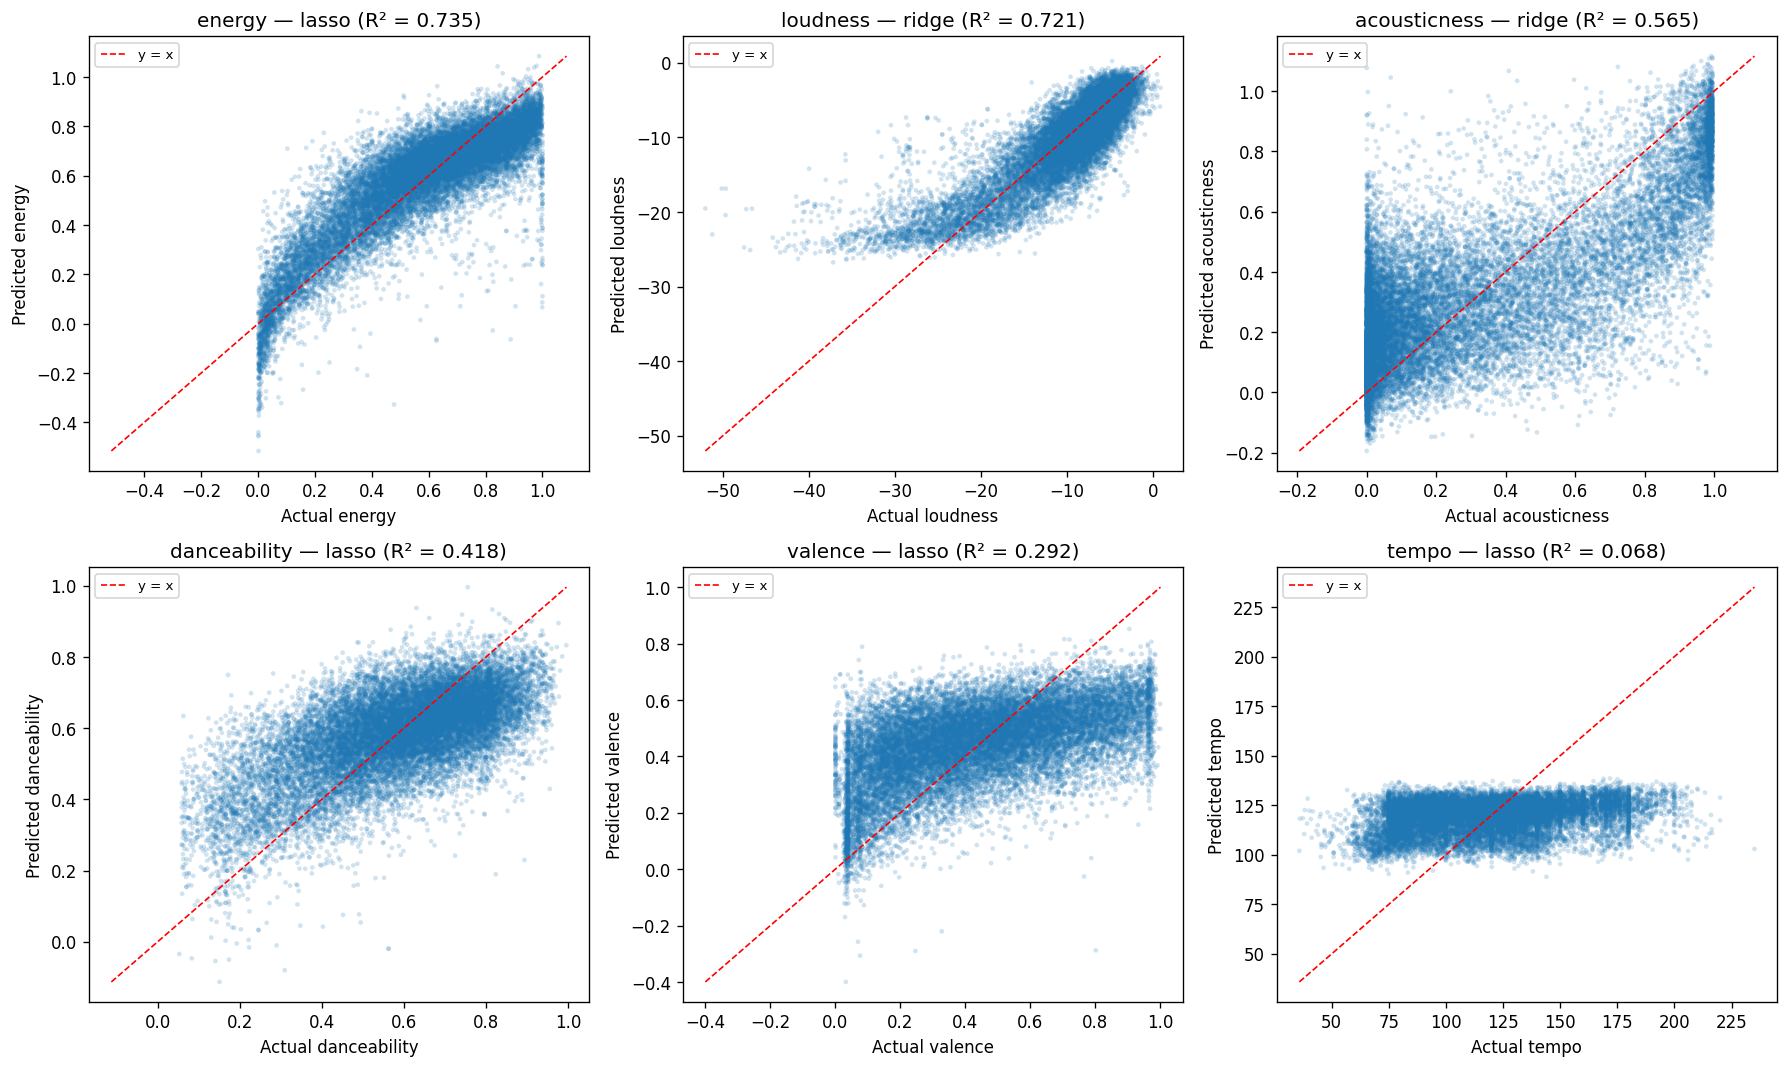
\includegraphics[width=\linewidth]{outputs/scatter_predicted_vs_actual.png}
\caption{Predicted vs.\ actual on the test set, best linear/regularized model per target. Dashed red line is $y=x$.}
\label{fig:scatter-linear}
\end{figure}

\begin{figure}[H]
\centering
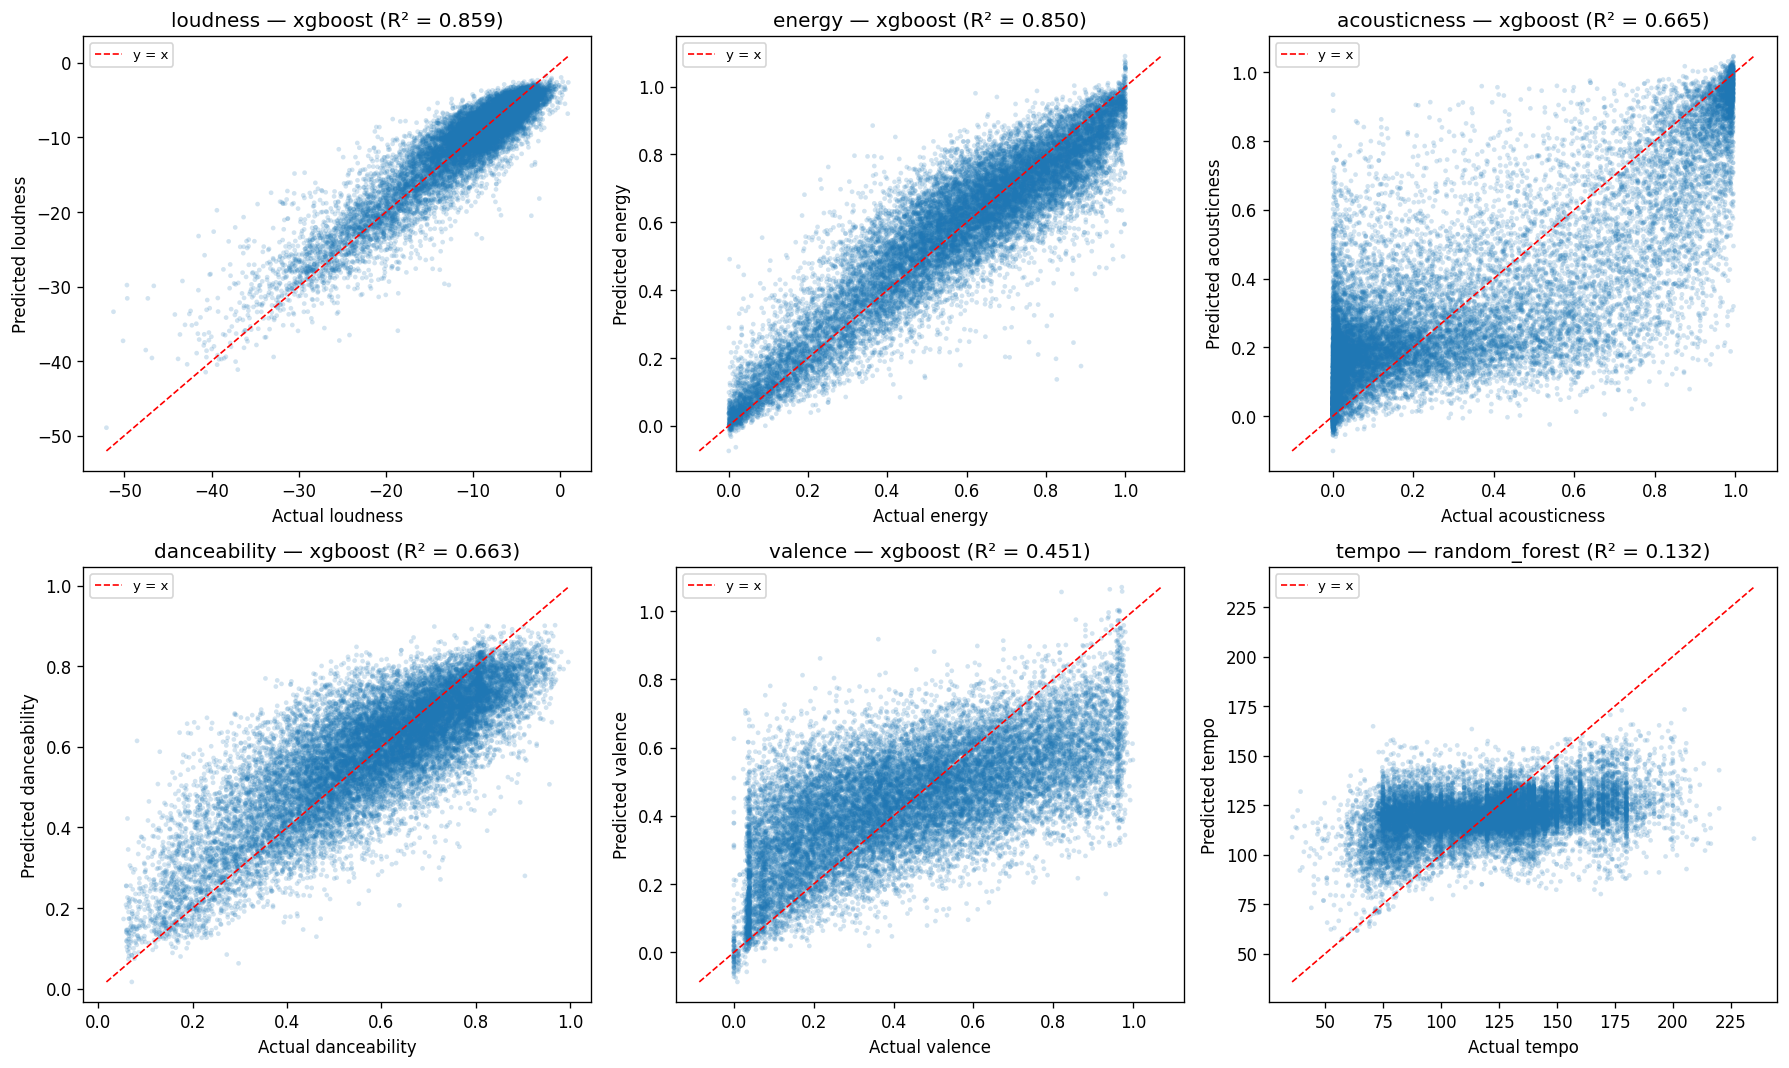
\includegraphics[width=\linewidth]{outputs/tree_predicted_vs_actual.png}
\caption{Predicted vs.\ actual on the test set, best tree-based model per target. Dashed red line is $y=x$. Compared to Figure~\ref{fig:scatter-linear}, scatter clusters noticeably tighter for \emph{danceability}, \emph{valence}, and \emph{acousticness}.}
\label{fig:scatter-tree}
\end{figure}

\subsection{Generalization}

A consistent concern with high-capacity models is overfitting to the training distribution. We check generalization by comparing held-out validation and held-out test $R^2$ for every (target, model) pair. The validation--test gap stays within $\pm 0.015$ across all $36$ combinations:

\begin{table}[H]
\centering
\caption{Range of validation $R^2$ minus test $R^2$ across the 6 proposal targets, by model family.}
\label{tab:gen-gap}
\small
\begin{tabular}{lrr}
\toprule
\textbf{model} & \textbf{min gap} & \textbf{max gap} \\
\midrule
linear / Ridge / Lasso & $-0.001$ & $+0.012$ \\
Random Forest          & $-0.007$ & $+0.014$ \\
XGBoost                & $-0.005$ & $+0.011$ \\
\bottomrule
\end{tabular}
\end{table}

Tree models do not generalize meaningfully worse than the linear family, and no model shows a gap large enough to suggest training-set memorization. The $R^2$ values reported in Table~\ref{tab:r2-pivot} are honest ceilings on what these features can achieve, not artifacts of hyperparameter tuning.

\subsection{Hyperparameter selection}

Optimal regularization strengths varied substantially across targets (Table~\ref{tab:alphas}), confirming that hyperparameter tuning was not vacuous. Notably, \texttt{LassoCV} selected its smallest available $\alpha$ ($10^{-4}$) for nearly every target, meaning that with $13$ features cross-validated MSE was always best when essentially no features were zeroed. We address this in Section~\ref{sec:redundancy} by sweeping $\alpha$ manually to extract a feature drop-off ranking.

\begin{table}[H]
\centering
\caption{Best regularization strengths from \texttt{RidgeCV}/\texttt{LassoCV} (5-fold).}
\label{tab:alphas}
\small
\begin{tabular}{lrr}
\toprule
\textbf{target} & \textbf{Ridge} $\alpha$ & \textbf{Lasso} $\alpha$ \\
\midrule
danceability & $8.53$    & $0.00010$ \\
energy       & $5.30$    & $0.00010$ \\
valence      & $22.12$   & $0.00010$ \\
acousticness & $8.53$    & $0.00010$ \\
loudness     & $5.30$    & $0.00013$ \\
tempo        & $148.74$  & $0.01125$ \\
\bottomrule
\end{tabular}
\end{table}

\section{Feature Redundancy Analysis}
\label{sec:redundancy}

The proposal frames feature redundancy as a primary research question. We approach it from two complementary angles: standardized Lasso coefficients (linear, sparsity-aware) and tree-model feature importances (nonlinear, interaction-aware).

\subsection{Lasso: standardized coefficients and feature drop-off ranking}

We rescale Lasso coefficients to fully standardized space (units of $\sigma_{\text{target}}$ per $\sigma_{\text{feature}}$) so magnitudes are comparable across targets with different native scales. Figure~\ref{fig:lasso-coef} shows the result. The reciprocal relationship between \emph{loudness} and \emph{energy} is strikingly visible: each is the dominant predictor of the other, with standardized coefficient $\approx 0.65$.

\begin{figure}[H]
\centering
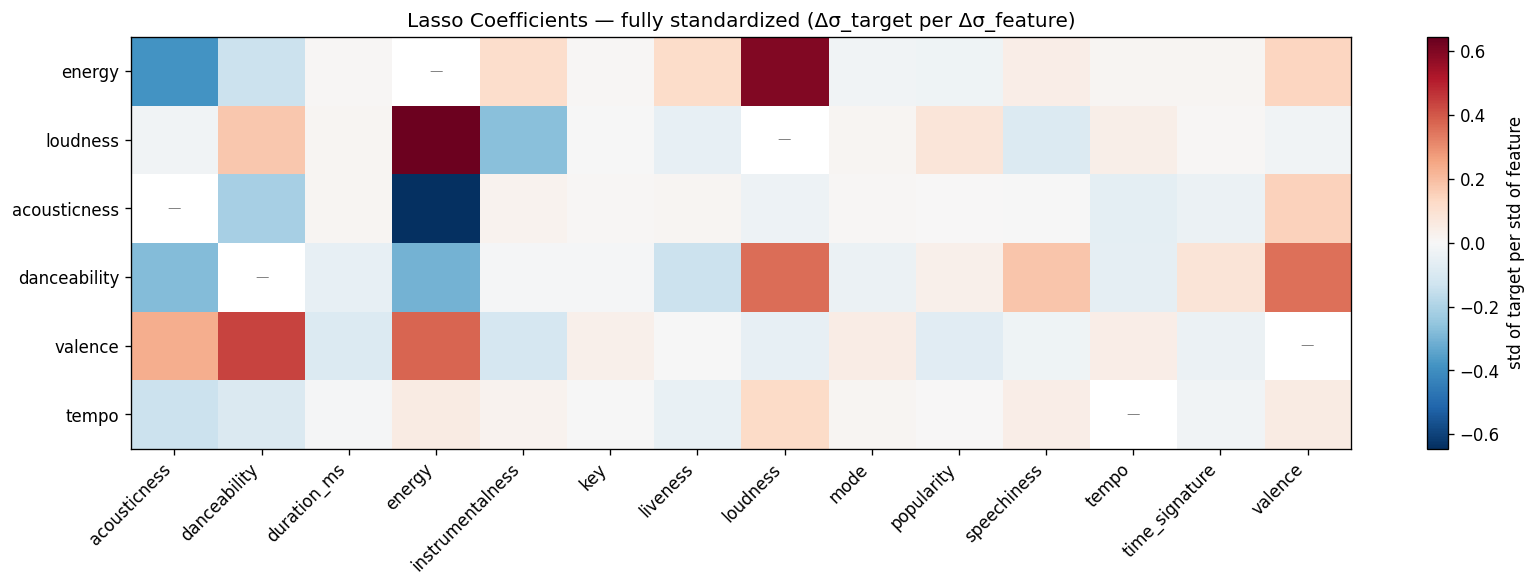
\includegraphics[width=\linewidth]{outputs/lasso_coefficient_heatmap.png}
\caption{Lasso coefficients in fully standardized space (rows: target; columns: feature). Red = positive, blue = negative, white cells indicate the diagonal (a feature cannot predict itself).}
\label{fig:lasso-coef}
\end{figure}

Because \texttt{LassoCV} preferred near-zero $\alpha$ at the optimum, we additionally compute a \textbf{Lasso path} per target: as $\alpha$ grows, features get zeroed in order of decreasing importance, and the order in which each feature first becomes nonzero is its \emph{essentiality rank}. Figure~\ref{fig:lasso-rank} sorts columns by mean rank across targets, so the most universally essential features appear on the left.

\begin{figure}[H]
\centering
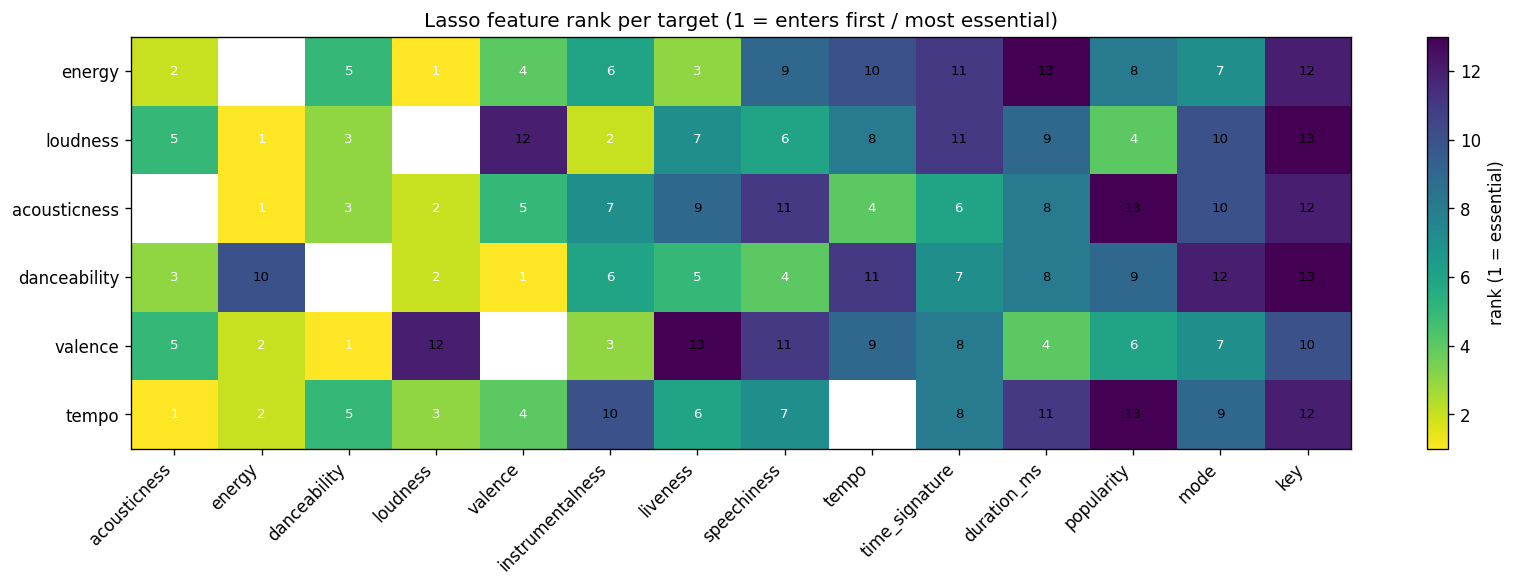
\includegraphics[width=\linewidth]{outputs/lasso_feature_rank_heatmap.png}
\caption{Lasso feature-essentiality rank per target ($1$ = enters first, most essential; $13$ = last to enter, most dispensable). Columns are sorted by mean rank across targets.}
\label{fig:lasso-rank}
\end{figure}

\subsection{Tree-based feature importance}

Both Random Forest and XGBoost expose normalized feature importances (each model's importances sum to $1$). Figure~\ref{fig:tree-imp} stacks the two as a pair of heatmaps. Both methods independently identify \emph{energy} and \emph{loudness} as the dominant predictors of each other ($\approx 0.55$--$0.77$), and identify \emph{energy} as the dominant predictor of \emph{acousticness}.

\begin{figure}[H]
\centering
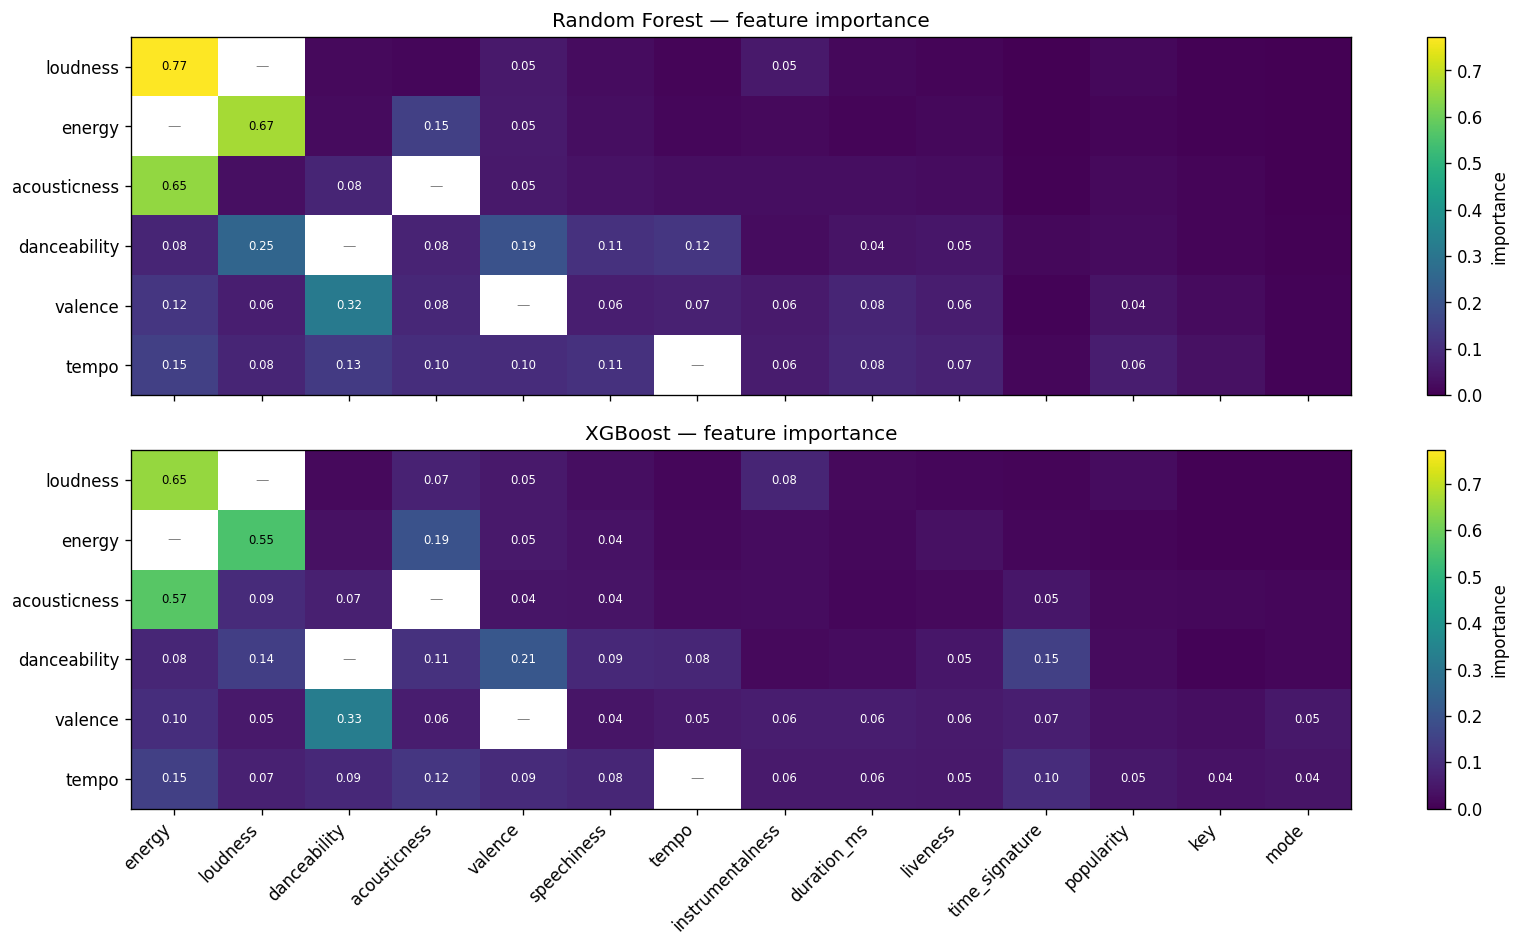
\includegraphics[width=\linewidth]{outputs/tree_feature_importance_heatmap.png}
\caption{Tree-model feature importance (RF and XGBoost). Both methods agree on the dominant predictors per target.}
\label{fig:tree-imp}
\end{figure}

\subsection{Cross-method agreement}

Each method produces a top-3 most important feature list per target. Table~\ref{tab:agreement} measures overlap between Lasso (linear) and XGBoost (nonlinear) top-3 lists.

\begin{table}[H]
\centering
\caption{Top-3 most important features by target: Lasso vs.\ XGBoost. ``Overlap'' counts shared features.}
\label{tab:agreement}
\small
\begin{tabular}{l p{4.4cm} p{4.4cm} c}
\toprule
\textbf{target} & \textbf{Lasso top 3} & \textbf{XGBoost top 3} & \textbf{overlap} \\
\midrule
loudness     & energy, instrumentalness, danceability & energy, instrumentalness, acousticness & 2 \\
energy       & loudness, acousticness, liveness       & loudness, acousticness, valence        & 2 \\
acousticness & energy, loudness, danceability         & energy, loudness, danceability         & 3 \\
danceability & valence, loudness, acousticness        & valence, time\_signature, loudness     & 2 \\
valence      & danceability, energy, instrumentalness & danceability, energy, time\_signature  & 2 \\
tempo        & acousticness, energy, loudness         & energy, acousticness, time\_signature  & 2 \\
\bottomrule
\end{tabular}
\end{table}

Linear and nonlinear methods agree on at least $2$ of the top $3$ most important features for every target, and on all three for \emph{acousticness}. This convergence across very different inductive biases is strong evidence that the redundancy structure is real, not an artifact of any single model class.

\section{Discussion}

\paragraph{A clear hierarchy of feature redundancy.} The most striking finding is the spread in test $R^2$ across targets: from $0.86$ for \emph{loudness} down to $0.13$ for \emph{tempo}. A flat ``high $R^2$ everywhere'' result would imply Spotify's audio features are uniformly redundant; a flat ``low $R^2$ everywhere'' result would imply they are uniformly independent. The actual hierarchy --- \emph{loudness} $\approx$ \emph{energy} $>$ \emph{acousticness} $\approx$ \emph{danceability} $>$ \emph{valence} $>$ \emph{tempo} --- says that \textbf{audio features carry overlapping information, but the overlap is concentrated in a few feature pairs}.

\paragraph{Loudness and energy are nearly substitutes.} Both linear coefficients and tree importances make this finding unambiguous: each is the other's dominant predictor, with magnitudes far above any other feature. Practically, this suggests that for tasks like playlist construction, ``high energy'' and ``high loudness'' are not two independent dials a DJ can turn --- they are largely the same dial measured twice.

\paragraph{Danceability is nonlinear.} The largest linear-to-tree improvement is on \emph{danceability} ($+0.245$ in $R^2$ from Lasso to XGBoost). This means \emph{danceability} is not a linear combination of other features; rather, it depends on \emph{interactions} (e.g., ``high valence \emph{and} moderate tempo \emph{and} not too acoustic''). This is consistent with the intuition that what makes a song danceable is hard to reduce to a single audio metric.

\paragraph{Tempo is the most independent feature.} Even XGBoost achieves only $R^2 = 0.13$ on \emph{tempo}, and feature-importance is diffuse rather than concentrated on any single predictor. The inability of any model class to recover \emph{tempo} from the other features, combined with the diffuse importance pattern, is strong evidence that tempo carries information not duplicated elsewhere in the feature set. This has a satisfying musical interpretation: songs of any tempo can be of any energy level (a slow ballad and a fast EDM track can both be ``intense''), so beats-per-minute is genuinely orthogonal to the other audio descriptors.

\paragraph{Linear vs nonlinear gap as a redundancy signal.} The size of the linear-to-tree improvement is itself a useful diagnostic. Targets with a small gap (\emph{loudness}, \emph{tempo}) have whatever redundancy structure they have already captured by linear methods; targets with a large gap (\emph{danceability}, \emph{valence}) hide their predictability in interactions among features.

\section{Limitations}

\paragraph{Single random seed.} All splits and stochastic models use \texttt{random\_state=42}. Differences in $R^2$ smaller than approximately $0.01$ should not be over-interpreted. Bootstrapped confidence intervals would tighten the comparisons but were out of scope.

\paragraph{No artist-level leakage control.} The same artist may appear in train and test splits, which can inflate $R^2$ on features artists tend to keep consistent (mastering loudness, characteristic tempo). A defensive variant would be \texttt{GroupKFold} on \texttt{artist\_name}; we did not run this.

\paragraph{No formal statistical testing.} We do not report confidence intervals on $R^2$, nor significance tests between competing models. Where two models are within $\sim 0.01$ of each other (e.g., RF vs.\ XGBoost on \emph{tempo}), the choice of ``best'' is essentially noise.

\paragraph{Default tree hyperparameters.} The Random Forest and XGBoost configurations are reasonable defaults rather than the result of nested cross-validation. A more rigorous tuning step might lift tree-model $R^2$ by an additional $0.01$--$0.03$, but is unlikely to change the qualitative ordering of targets.

\paragraph{Single dataset, single feature schema.} Our claims about ``Spotify's audio features'' are limited to the schema used in this Kaggle release. Spotify's modern API exposes a slightly different set, and additional features (e.g., key signatures, harmonic descriptors) might further explain \emph{tempo}.

\section{Conclusion}

We trained six regression models across six target audio features, evaluated them with three metrics on a held-out test set, and used both linear coefficient and tree-importance methods to identify which features explain which. Our pipeline runs reproducibly from cleaned data to final tables in five sequential notebooks (\texttt{dataclean.ipynb} $\to$ \texttt{baseline.ipynb} $\to$ \texttt{regularized\_models.ipynb} $\to$ \texttt{tree\_models.ipynb} $\to$ \texttt{final.ipynb}).

The substantive finding is that Spotify's audio features form a redundancy hierarchy, with \emph{loudness} and \emph{energy} essentially substitutable, \emph{acousticness}/\emph{danceability}/\emph{valence} moderately predictable from the rest, and \emph{tempo} largely independent. This result holds across linear and nonlinear model classes and across two different feature-importance methodologies, and it is robust to the validation/test boundary (gaps below $\pm 0.015$). For downstream applications such as playlist construction, the practical implication is that a small number of features (\emph{energy} or \emph{loudness} as a stand-in for both, plus \emph{tempo} as a genuinely independent axis, plus one of \emph{valence} or \emph{danceability} for ``mood'') captures most of the variation Spotify tracks --- the remaining features are largely refinements rather than independent axes.

\section*{Reproducibility}

All code, data splits, and outputs referenced in this report are produced by the notebooks in the project repository. To reproduce: install dependencies via \texttt{pip install -r requirements.txt} and run the five notebooks in the order listed in the Conclusion. Every figure in this report corresponds to a PNG in \texttt{outputs/}.

\end{document}
